\documentclass{sigchi}

% Use this command to override the default ACM copyright statement (e.g. for preprints). 
% Consult the conference website for the camera-ready copyright statement.


%% EXAMPLE BEGIN -- HOW TO OVERRIDE THE DEFAULT COPYRIGHT STRIP -- (July 22, 2013 - Paul Baumann)
% \toappear{Permission to make digital or hard copies of all or part of this work for personal or classroom use is 	granted without fee provided that copies are not made or distributed for profit or commercial advantage and that copies bear this notice and the full citation on the first page. Copyrights for components of this work owned by others than ACM must be honored. Abstracting with credit is permitted. To copy otherwise, or republish, to post on servers or to redistribute to lists, requires prior specific permission and/or a fee. Request permissions from permissions@acm.org. \\
% {\emph{CHI'14}}, April 26--May 1, 2014, Toronto, Canada. \\
% Copyright \copyright~2014 ACM ISBN/14/04...\$15.00. \\
% DOI string from ACM form confirmation}
%% EXAMPLE END -- HOW TO OVERRIDE THE DEFAULT COPYRIGHT STRIP -- (July 22, 2013 - Paul Baumann)


% Arabic page numbers for submission. 
% Remove this line to eliminate page numbers for the camera ready copy
% \pagenumbering{arabic}


% Load basic packages
\usepackage{balance}  % to better equalize the last page
\usepackage{graphics} % for EPS, load graphicx instead
\usepackage{times}    % comment if you want LaTeX's default font
\usepackage{url}      % llt: nicely formatted URLs

% llt: Define a global style for URLs, rather that the default one
\makeatletter
\def\url@leostyle{%
  \@ifundefined{selectfont}{\def\UrlFont{\sf}}{\def\UrlFont{\small\bf\ttfamily}}}
\makeatother
\urlstyle{leo}


% To make various LaTeX processors do the right thing with page size.
\def\pprw{8.5in}
\def\pprh{11in}
\special{papersize=\pprw,\pprh}
\setlength{\paperwidth}{\pprw}
\setlength{\paperheight}{\pprh}
\setlength{\pdfpagewidth}{\pprw}
\setlength{\pdfpageheight}{\pprh}

% Make sure hyperref comes last of your loaded packages, 
% to give it a fighting chance of not being over-written, 
% since its job is to redefine many LaTeX commands.
\usepackage[pdftex]{hyperref}
\hypersetup{
pdftitle={SIGCHI Conference Proceedings Format},
pdfauthor={LaTeX},
pdfkeywords={SIGCHI, proceedings, archival format},
bookmarksnumbered,
pdfstartview={FitH},
colorlinks,
citecolor=black,
filecolor=black,
linkcolor=black,
urlcolor=black,
breaklinks=true,
}

% create a shortcut to typeset table headings
\newcommand\tabhead[1]{\small\textbf{#1}}


% End of preamble. Here it comes the document.
\begin{document}

\title{Visualisation of Formula One Racing Results}

\numberofauthors{3}
\author{
  \alignauthor Giuseppe Callari\\
    \affaddr{\normalsize Katholieke Universiteit Leuven}\\
    \email{\normalsize  giuseppe.callari@student.kuleuven.be}\\
  \alignauthor Michael Vincken\\
    \affaddr{\normalsize Katholieke Universiteit Leuven}\\
    \email{\normalsize michael.vincken@student.kuleuven.be}\\
  \alignauthor Stefan Pante\\
    \affaddr{\normalsize Katholieke Universiteit Leuven}\\
    \email{\normalsize stefan.pante@student.kuleuven.be}\\
}

\maketitle

\begin{abstract}
This paper describes the design and implementation of a visualisation of Formula One racing results. The user can interact with the visualisation using a draggable timeline. We use coloured bar charts for a visual representation of the strengths and weaknesses of specific drivers or constructors over the years. Moreover, our visualisation gives the user the opportunity to compare two drivers based on their finishing positions per season. Through this paper, we will shortly discuss the problems we have encountered such as the point system for the championship that has been changed several times over the years and that the original data format did not allow for a performant visualisation, which required us to do some heavy preprocessing on the data. At the end of this paper we describe some lessons we have learned in the process of making this visualisation such as the drawing order of SVGs in D3.js and assumptions that were made but were not always correct.

\end{abstract}

\keywords{
Information visualisation; Formula One; Race results; Motor sport; Seasonal wins; Drivers; Constructors;
}

\category{H.5.m.}{Information Interfaces and Presentation (e.g. HCI)}{Miscelaneous}

\begin{figure}
\begin{center}
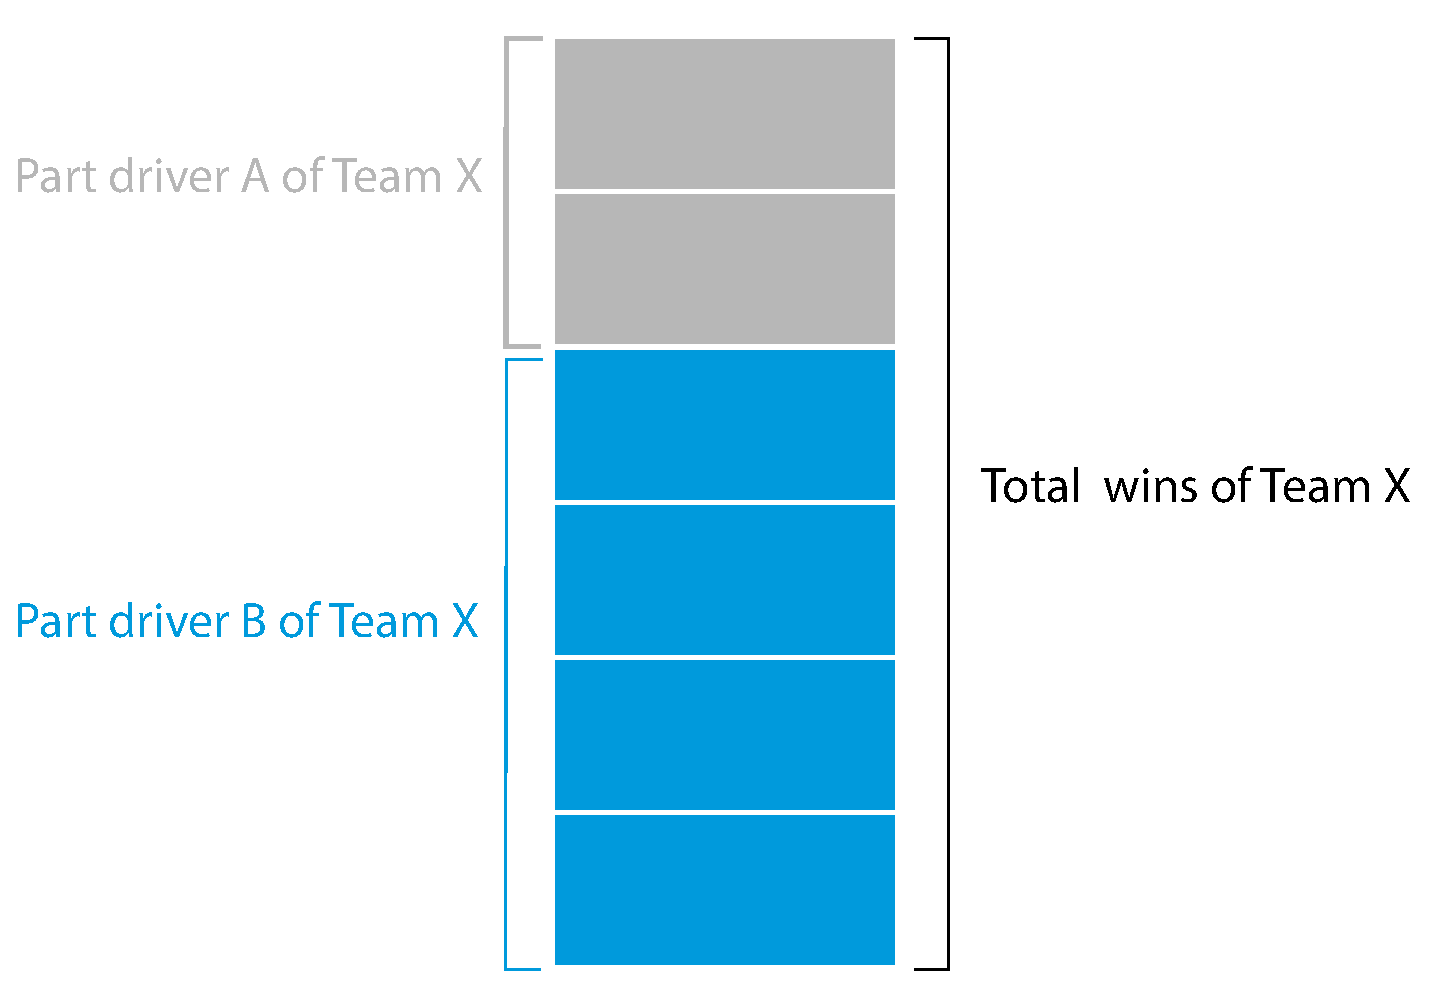
\includegraphics[width=\columnwidth]{images/stackedbar.pdf}
\end{center}
\end{figure}

\section{Introduction}
The FIA Formula One World Championship, better known as Formula One or F1, is one of the most popular motor sports in the world. The F1 season consists of a series of races, also called Grands Prix, held throughout the world. Each season consists of a certain number of races. During a season, a number of teams or constructors (we will use these names interchangeable in this paper) compete with each other. Each team consists of two drivers and some additional secondary drivers. It is important to note that a team may only use two cars during a race. After each race, drivers receive points depending on their finishing position. In the current system, the top ten driver-car combinations are awarded points. Based on the racing result of the drivers at the end of the season, the team with the highest cumulative score wins the constructors title and the driver with the highest individual score wins the World Championship title.
 
There already exist visualisations for consulting the statistics of Formula One racing results[1][2]. Most of these visualisations give the user an overview of results per season. The specific focus of our visualisation is that we want to make it easy to compare driver (or constructor) results over several years.
 
The goal of this visualisation is to present an overview of seasonal race results for specific drivers throughout their active years, while keeping an overview of the opponents. This visualisation is interesting for motor sport fanatics or those who want to know more about driver performance.
 
In this paper, we first give some background information about Formula 1 racing statistics. Next, we describe the data set we used for our visualisation. Then we discuss the technology used for the visualisation. Then we describe the different parts of our visualisation. Finally, we discuss some related work. 



\section{Formula One Racing Statistics}

As stated previously, a Formula One racing team consists of several drivers. In general, two drivers are the main drivers of the team. The other drivers are test drivers or can take the place of one of the two main drivers in case one is not able to participate in a race (due to medical conditions or a disqualification). Each driver can earn points in a race when finishing in the top 10. In the current point system, the winner gets 25 points, the second 18 points, third 15 and so on. It is import to note that the scoring system has been changed several times over the years. This complicates comparing drivers or constructors over the years. This is why we choose to discard the original points that each driver has earned and used the current point system for all drivers instead.


\section{Data Set}
For our visualisation, we made use of the Ergast API [REFERENTIE]. The Ergast API provides data for the Formula One and Formula E series from the beginning of the world championships in 1950 and 2015 respectively. Data can be requested in different formats: XML, JSON and JSONP. We opted to use JSON because it can be directly used in javascript without the need of parsing. 

A problem we encountered was that the Ergast API only provides data about the lap times starting from 2008. We did not find any other source which provided this kind of information. To overcome this problem we decided to focus on driver and constructors performances through the years. This data was readily available because the API supports requests for statistics per race or per, season for both the drivers and the constructors. Despite not containing all the data we originally wanted, the Ergast API was the most detailed source of Formula One statistics we could find without resorting to building  a web scraper. 

The API was used to build our own static dataset. A direct connection between the visualisation and the API was not possible due to the multitude of requests necessary to get all required data. This would result in unacceptable slow behaviour. More about how we used the API to build our own dataset is detailed in section [REFERENTIE]. 

\section{Our Visualisation}
Our visualisation consists of three parts as shown in Figure [REFERENTIE]: the timeline is the main part of our visualisation where we provide an overview of seasonal wins (or scores) for the different drivers and constructors. The second part, situated under the timeline, focuses on two specific drivers to enable a comparison of their performance.  

\subsection{Timeline}

The timeline contains the active years of the selected driver. For each year, we plot the number of wins using bar charts. Each individual bar represents a constructor who competed for the title in that specific year. Figure 1 illustrates that a bar is divided in two colours, namely blue and grey. The blue bar, the bottom part, represents the number of wins of the driver who performed the best for that team. More specifically, this bar represents the driver who has earned the most points or wins – depending on the selected criteria – during the season. The grey bar, the upper part of the bar, represents the number of wins of his opponent from the same team. These two bars are stacked on top of each other. In this way, we visualise the individual wins of the drivers, but also the number of wins for a constructor. 
 
Another reason why we visualised the scores like this is to enable interaction with the user. At first the user selects a driver in the bottom part of the visualisation, e.g. Vettel. The lower part of the visualisation is now updated with the data of Sebastian Vettel. When the user now hovers over a part of a bar in the upper part (as discussed above), a tooltip pops up and displays the name of the corresponding driver, as well as his number of wins.  By clicking on that part of the bar, the data of the corresponding driver is loaded and the visualisation in the lower part is updated. 

Our timeline is in fact a two-dimensional graphic with one dimension used to represent time and the second to represent a magnitude associated to the events represented. In our visualisation, the events are the performances of drivers. According to J.Y Blaise et al.[9] , this representation of time is easy to read; it usefully enhances comparisons, cross examination of indications, and allow for magnitude assessment.  Furthermore, they call this kind of timeline a time chart. 

\paragraph{Alternatives} % (fold)
\label{par:alternatives}
Cleveland et al.  [10] prefer to replace stacked bar charts by grouped dot charts. This makes comparing drivers of a same team easier: length judgements are replaced by position judgements. However, we already sort drivers belonging to the same team: the best driver is placed at the bottom, if the team does not contain a selected driver. If a selected Selected drivers driver is present, he is placed at the bottom instead.are always placed on the bottom. This ordering already makes the ordering of drivers in a team clear. Hovering is used to reveal the points or wins of a driver. Furthermore, if we replaced the stacked bar charts by grouped dot charts, more space would be is needed on the axis that represents timein the time dimension. 

% paragraph alternatives (end)


\subsection{Navigator}

A draggable bar is added beneath the timeline for easier navigation (see figure XX), called the navigator. Inside the navigator, a miniature version of the bar charts for each year is displayed to give a quick overview. A draggable slider is placed on top to navigate through the years.
This miniature version shows the timeline as a whole, from the beginning to the end without sideways scrolling. This provides an overview for the user. The miniature version does not aim to provide all the information to the user, but it rather is an incentive for the user to explore certain periods. 

It could for example trigger the user to drag the navigator to the start of some driver’s career when exploring the end of it. The start could have same peaks which the user did not remark on the visible section of years selected period of the main timeline. The miniature version only shows the bars of the non selected drivers and selected drivers in the corresponding colors as in the main timeline. Visualizing the distribution of the data and showing individual data values in the navigator is proposed by Stephen G. Eick[11]: “Linking sliders to the data they control suggests many natural and obvious extensions.”


\paragraph{Alternatives}
We considered two alternative representations for the navigator in which the bar charts are replaced or accompanied by a miniature version of the trendline for the two selected drivers. A drawback of the usage of the trendline is that the difference between the performance of the drivers over the years becomes less obvious because of the small scale of the navigator. Another drawback is obvious if we only use the trendline: the information about the drivers other than the selected is lost.
 We show a mock-up of this navigator in figure [REF] and compare it with our version in figure [REF]. We believe this alternative duplicates less shown data, but withholds valuable informatio from s the user  valuable information to help him exploring the data e.g. peak performances of non selected drivers will not be as visible.


\subsection{Comparing two drivers}
The user can compare two drivers based on their finishing positions. In order to get an overview, the user clicks on part of a bar, as described above. Now the number of times the driver has finished first, second and third pops up. When the user clicks on another part of a bar, the same statistics are placed next to the statistics of the first driver. In this way, one can simply compare the performances of the two drivers. When the users clicks another part of a bar, the driver that was selected first will disappear and be replaced by the last selected.

An alternative functionality considered is the following: hovering over a bar lights up all bars corresponding to the same driver. It makes the user clear which driver he/she will select. The user gets an overview in what teams the hovered driver has participated. Not all lit up bars are label shown with their label, but this view gives the user an idea in what kind of teams the driver participated and if he was dominant in these teams. For more details, the driver must be selected.

\subsection{Statistics}

Below the main timeline and the navigator, another section is visualised in parallel. This line is divided in year blocks similar to the main timeline. In every block, more information about the selected chosen drivers is shown. These blocks are reserved preserved for analysis of the selected drivers only. Three metrics are compared: number of first places, number of second places and number of third places. These correspond to rankings for which a driver is allowed on the podium during the podium ceremony. During this ceremony, the best three drivers are celebrated after each race. The best racer, the one who won the race, receives its price. Nowadays, the second and third driver also receive something as souvenir for their achievement. These prices and souvenirs differ throughout the history of this motorsport.  Podium finishes are considered an important statistic used in sports to analyse an athlete's career (or driver's career in motorsport). Achieving a podium finish puts the driver in the spotlights by honoring its achievement publicly. During the olympics, medals and thus podium places are an important metric as well. Countries are usually ranked by the number of medals achieved by their athletes [REFERENTIE]. MotoGP, the premier class of GP motorcycle racing, [REFERENTIE] provides a search functionality on its official website in order to let user explore their database of races, drivers and results. ``Podium with riders of the same nation'' is a search space users can explore.

For each podium finish place (first, second and third), the number obtained during that season achieved is visualised using circles. The number of circles indicate the number achieved for a place. The color of a circle corresponds to the driver. Each place has two horizontal rows of circles, in which each driver corresponds to a row. This design decision facilitates comparison of two drivers for these metrics. (grouping, color, discrete values etc referenties). Furthermore, in this block, the names of the teams of the drivers made part of are shown as well. Place and color of the constructor in the statistics block indicate who is the corresponding driver. The position in the block corresponds to the position of the name of the driver shown in the left upside corner of the visualisation.  Events like team switches or temporary stops are visualised this way. These events are thus implicitly visualised., instead of explicitly shown  the user where a selected driver switched constructor. Next to each team, a medal is shown to indicate the final ranking for the corresponding year. A first place and thus championship win is decorated with a gold medal, a second place is decorated with a silver medal, a third place is decorated with a bronze medal and a place lower than three is decorated with a dark blue medal. In each medal, the number corresponding with the finishing position in the championship place is shown. We believe the podium metrics provide context for the results (points or wins) shown on the main time concerning the selected drivers. We already mentioned in section [REFERENTIE] which discusses the dataset that a significant amount of drivers have gathered points in a year, but did not achieve a single victory. Let us consider drivers who achieved no or very few (one or two) wins. These drivers however could have achieved many podium places during a year. Second and third places have always be rewarded by points [REFERENTIE]. This could trigger the user to switch to the points view for the main timeline to further investigate the selected drivers.
\section{Lay Out}
As shown in figure [INSERT REF] and as discussed in section [REF], our visualisation consists of three parts: The timeline, the navigator and the statistics. The navigator lies between the statistics and the timeline. Notice that the statistics are shown parallel one-on-one with the corresponding bar chart blocks. Thus the number of statistics blocks are equal to the number of bar chart blocks. The navigator has the role to summarize and give an overview of the carreers of the selected drivers. It does not have the role to show details, but can show significant raises and drops in the careers of the selected drivers. This gives the user the possiblity to remark these significant changes, even if the selected view does not cover the corresponding years. 

The reason we put the navigator between the statistics and the timeline, has no hard foundation based on design patterns proposed and accepted by the information visualisation community. The design decission is based on the conceptual difference of the statistics and the timeline. The navigator splits these two parts. Furthermore, since we have the goal to visualize careers of drivers between 1950 and 2015 [TRUE?], the navigator has a central role in the visualition and we want to present it this way by centralizing it.

This was not percepiated the same way by experts during the final presentation of this visualisation. Alternatives for the lay out are presented in figures [REFONE] and [REFTWO]. Figure [REFONE] respects gives rise to a more hierarchical, top down order in which the navigator presents the overview in miniature. Below the navigator, details are shown of the selected period. We present the statistics as information which provides context to the timeline, the backbone of our visualisation. It is also possible to put the timeline on the bottom of the visualisation, which breaks the hierarchical concept explained at first. This layout however separates the navigator from the timeline and the statistics, like the first alternative. 


\subsection{Points vs wins} % (fold)
\label{sub:points_vs_wins}
In the initial design of our visualisation number of wins were used to determine the height of the bars of the different drivers. We opted to use the number of wins of a driver in order to compare drivers because this metric that has not been changed over the years. In contrats with In contrary to the number of wins, the score system has changed several times over the years [REFERENTIE tabel Wikipedia]. Therefore, this metric is not ideal to compare drivers in the main timeline which competed in different periods. To overcome this problem we normalised the score systems to the system used in the year 2014. This way we give the user the opportunity to compare two drivers based on their points. As described in paragraph [REFERENTIE] a driver who has won the most races does not always has the most points and therefore did not win the championship of that year. The user can now easily switch between the points and wins of the selected drivers to review their season. We believe that the statistics beneath the timeline provide the context to interpret results of drivers and that they can be an incentive to change the view, as discussed in statistics.
% subsection points_vs_wins (end)

\subsection{Layout} % (fold)
\label{sub:layout}
As shown in figure [INSERT REF] and as discussed in section [REF], our visualisation consists of three parts: The timeline, the navigator and the statistics. The navigator is positioned between the statistics and the timeline. Notice that the statistics are positioned beneath the timeline and that each block in the statistics corresponds to a year in the timeline. 
The navigator has the role to summarize and give a global  overview of the careers of the selected drivers.I It does not show a detailed view, but can be used to pinpoint interesting events in a driver’s career by displaying  significant raises and drops in the careers of the selected drivers. This gives the user the possibility to remark these significant changes, even if the current visible section of the timeline does not cover the corresponding years.

The reason we put the navigator between the statistics and the timeline, has no hard foundation based on design patterns proposed and accepted by the information visualisation community. The design decision is based on the conceptual difference between  the statistics and the timeline. The navigator is used as a separation between these two parts.

This was not perceived the same way by the visualisation experts during the final presentation of the visualisation. Based on their feedback,alternatives are considered for the layout. See figure [REFONE]. The first alternative shows the navigator at the top. This representation shows a more hierarchical, top down order in which the navigator presents a global overview. Below the navigator, the timeline shows a more detailed view on the data. At the bottom, the statistics are shown. They show even more detail and provide context to the timeline, the backbone of our visualisation. 

Another alternative is to put the navigator at the bottom of the visualisation, which would cause the detailed view of the timeline and statistics to presented at the top and the global overview to be positioned at the bottom. The first alternative seems to be the better if we adhere to the principal of overview first (REFERENTIE NAAR OVERVIEW FIRST: The Eyes Have It: A Task by Data Type Taxonomy for Information Visualizations ).

The Budgets Forecasts discussed by Edward Segel et al. [12] present a slider, placed on the bottom, to navigate through the years.  This navigation does not correspond to ours: when sliding from past to present, the line graph is more and more revealed. If the slider is put on present, the whole graph is shown. Hovering over the graph reveals details-on-demand, a design principle we also respected, as discussed in section [TIMELINE SECTION].

Furthermore, sliding our navigator zooms in to the selected period of time. Thus, the whole visualisation respects the overview first, zoom and filter, then details-on-demand design principle.
% subsection layout (end)
\section{Implementation} % (fold)
\label{sec:implementation}

The implementation of the visualisation consists of five parts: data gathering, the navigator, the timeline and the statistics.

\subsection{Data gathering} % (fold)

We used the Ergast F1 API to gather our data. We originally planned to connect directly to the API to retrieve the necessary data. It quickly became apparent that a direct connection was not suitable because of the structure of the API. Because our visualisation aggregates a lot of data, too many requests would be required, which would have resulted in very poor performance, numerous time-outs and overall, a worsened user experience. After downloading a database dump, the reasons for the bad performance were immediately clear. The relational database was heavily normalised, requiring multiple joins for each API call we made. We opted to transform the data to a JSON-object representation, which is downloaded in its entirety every time a user accesses the visualisation. We choose this approach instead of using a backend NoSQL database because we strongly believe such a database would not provide additional benefits to our users and we wanted to adhere to the KISS principle.

We developed a Node.js and python script to collect our data. These scripts automate the collection and transformation of our data. The drawback is that the scripts should be run each week to keep the data up-to-date, a process which also could be easily automated on a server.
\label{sub:data_gathering}

\subsection{Navigator} % (fold)
\label{sub:navigator}

The navigator is implemented without using a specialised library. Plain JavaScript in combination with jQuery in order to manipulate CSS, was sufficient to code the navigator. The miniature timeline, which shows all the bar charts (selected and not selected drivers of all the years)  has not all the functionality the main timeline provides: the stacked bars are not clickable and thus navigable, they are not hoverable and there are no trendlines for the selected drivers visualising the up and downs of their careers. The aforementioned functionalities are not only redundant for the mini timeline, but interfering too when navigating  through the timeline: clicking on a year in the mini timeline redirects the navigator to the clicked year in order to visualise the corresponding period. An unintentional click on the bars would trigger the switching scenario. 

Therefore, the code is not the same as the code for the main timeline. Making the code reusable, and thus avoiding code duplication, resulted in conflicts between svg-elements which were easily fixed by just duplicating the d3 code for the timeline. After duplication, refactoring followed in order to scale and place the miniature timeline under the navigator and in order to remove redundant functionality. 


\subsection{Timeline} % (fold)
\label{sub:timeline}
The timeline which holds all the bar charts is the backbone of our visualisation and its functionality is completely implemented using the d3.js framework. First, the data concerning the not selected drivers is visualised: these are represented by the grey stacked bar charts. Subsequently, the selected drivers are plotted, in a different color. Note that for a stacked bar with no selected driver involved, the lower bar represents the best driver in a team and the upper one the one who collected the least number of championship points. We believe that designing the non selected drivers in this way results in a more consistent visualisation. Making the stack order random would be a confusing factor and could interfere with our goal of visualising information in a clear way. This decision however has a consequence for our gathered data. The data concerning the selected drivers and all drivers who competed in the same years is processed and manipulated before it is visualised: the drivers of a team are sorted by the number of wins for each year. This is not done in the data gathering step, but processing the data after gathering them takes care of this sorting step.

After this step, the selected drivers are visualised on the timeline. The bars representing the selected drivers have a different color than the non-selected ones and are always shown as the bottom bar in a team, even if a non selected team-mate had most wins in the team. The performances based on the criterium of wins are represented by the height of the bars corresponding to the drivers. When two drivers are selected, the visualisation puts these two in focus by giving their bars a different color. It's tolerable if two not selected drivers cannot be easily compared because one is a non-dominant driver and thus the highest bar on a stacked bar. Details are provided by hovering on the bars. The bars of drivers in focus however must start at the same height (the bottom) to compare their heights. Starting at the bottom has the consequence that the performance can be read on the provided vertical axis.


A second consequence is that the line charts complement the bars of the selected drivers. The lines hit the top of the bars of the selected corresponding drivers.

To show which bar corresponds to which driver, we implemented tooltips using the library d3-tips [17] written by Justin Palmer.
When hovering over a bar, the bar lights up and the name of the corresponding driver is shown together with the amount of wins and the team to which it belongs.


\subsection{Statistics} % (fold)
\label{sub:statistics}

The process of creating and displaying the statistics underneath the timeline is handled by a template engine.Traditionally, the programmer would create new elements by building a string representation of the HTML required and appending it to the DOM. The template engine automates this process, which allows the developer to separate HTML from javascript. 

There are multiple template engines available. Two well known examples are Handlebars[ref]  and EJS[ref]. We opted for the EJS template engine because it allows for complex javascript statements inside a template, while Handlebars does not allow complex statements by default. 
voetnota (REFS toevoegen)

Information about the two drivers’ championship position, wins, second and third places for each year are given as input in the template engine as a JSON object, together with an URL pointing to the template. The output of the template engine is a representation of the statistic in string format that can easily be appended to the DOM.

\section{Lessons Learned}
When implementing the visualisation, we have dealt with some bottlenecks by not coding as generic as possible. For example, the overview shown in the navigator is implemented by reusing code of the timeline, keeping in mind that not all functionality (hovering, tooltips, selecting a new driver…) of the timeline must be supported by the navigator. During development, changes were made to our timeline. These changes were not forwarded to the navigator, which needed to be refactored. This was time consuming.
\section{Related Work} % (fold)
\label{sec:related_work}

\section{Future work} % (fold)
\label{sec:future_work}
An idea we got during our final presentation was to add the trendline from the main timeline in the navigator. This way the user could directly see where the selected driver has won a lot of races or has scored a lot of points. We have made a mock-up with real data in order to try out this idea [REFERENTIE]. In the end we concluded that this kind of visualisation technique was not very helpful in detecting interesting moments in a driver’s career. This is due to the height of the navigator. This in combination with the wavy form of the trendline does simply not give a good indication in difference of performance for one driver.
More detail about the wins, second and third places in the statistics can be shown. We could add the grand prix for each of the these places by creating a hover function (zie figuur blabla).
% section future_work (end)
\section{Related Work}
For related work, we focus on visualisations that represent an overview of results from team sports, e.g. basketball, football, soccer, cycling and so on.  
The FIFA Ranking For The Gulf National Teams[1] by Marcelod uses a hemisphere to represent a timeline with all the years in which a championship was organised. The y-axis represents the position of the soccer teams at the end of a season. This is an interesting way for visualising scores throughout the years. Marcelod used data from 1993 until 2014 to visualise 20 years of soccer championships. Our data ranges from 1960 until 2015. Therefore, we opted that it’s clearer to use a draggable timeline instead of a hemisphere. The user can interact with our timeline by using the navigator. In addition, Marcelo also uses "events" - these are the long vertical blue lines representing the various world cups - to divide the visualisation into regions. [This is a feature that we have also implemented in our visualisation, to indicate the year where a pilot has changed teams.] 
 

Another interesting visualisation is the Formula 1 Lap Charts by Davidor, which also relies on the Ergast web service for the dataset. This chart visualises the performance of the Formula 1 pilots in the first Grand Prix of the year. The x-axis includes a vertical line for each lap of a specific race. When we expand this visualisation for one full season instead of one race we can clearly see the fluctuations in the scores of the pilots. By following one line you can see the switches in position for that driver. These fluctuations are very interesting to get an overall view of the performances of certain drivers. We used this kind of visualisation as well for our trend line .

As discussed in the Lay Out section, The Budgets Forecasts discussed by Edward Segel et al. [12] makes use of a slider to navigate from past to present. But instead of focussing on a period of time, the line chart is more revealed as the user navigates to the present.



Spenke et al. [14] visualised Formula One racing results of the last 20 years using a visualisation tool called InfoZoom. This tool is not dedicated to visuations of Formula One data, but is generic and can be used to visualise any relational database. This tool visualises more data than our visualisation e.g. our visualisation does not visualise starting positions. However, it generally uses numbers and horizontal lines to show data. We use stacked bar charts in which bars of selected drivers are colored, line charts and circles in the statistics. Details-on-demand are achieved by using tooltips in our visualisation. In figure [REF], a Compressed Table Mode view is shown.


Burch et al. [15] present Timeline Trees to visualise transactions between elements. As an example, they visualised a football game between Germany and the Netherlands during the 1990 World Cup. This technique could be applicable on data of a single race or a single championship, in which position switches are visualised. For yearly data, which we use, using this technique seems more difficult since each season does cover the same drivers. 

A visualisation discussed in [ref], presents an overview of all records for summer Olympic events, in which every circle corresponds to a record. Details about a record are shown when hovering over it. We use the stacked circle approach to visualise the number of first, second and third places. Showing details about a podium finish by hovering over it, is future work.  

Blaise et al. [9] describe the evolution of their approach the visualise the city of Kraków and the changes it endured over time. In a first approach, navigating using their timeline showed a view of Kraków corresponding to the selected year. This design did not make it possible to compare two years since only one was shown. 

\section{Conclusion} % (fold)
\label{sec:conclusion}
In this paper we described the process for developing our visualisation about Formula One racing results, which consists of three parts. Using the navigator, the user can slide through time in order to compare two selected drivers. All the drivers and constructors are visualised by stacked bar charts in the timeline, the backbone of the visualisation. These bars either show the number of wins or gathered points. The metric can be switched by the user. Extra statistics are used to provide context to the visualised data in the timeline. For each part, alternatives are considered and discussed.
% section conclusion (end)


% section related_work (end)
% Balancing columns in a ref list is a bit of a pain because you
% either use a hack like flushend or balance, or manually insert
% a column break.  http://www.tex.ac.uk/cgi-bin/texfaq2html?label=balance
% multicols doesn't work because we're already in two-column mode,
% and flushend isn't awesome, so I choose balance.  See this
% for more info: http://cs.brown.edu/system/software/latex/doc/balance.pdf
%
% Note that in a perfect world balance wants to be in the first
% column of the last page.
%
% If balance doesn't work for you, you can remove that and
% hard-code a column break into the bbl file right before you
% submit:
%
% http://stackoverflow.com/questions/2149854/how-to-manually-equalize-columns-
% in-an-ieee-paper-if-using-bibtex
%
% Or, just remove \balance and give up on balancing the last page.
%
\balance

\bibliographystyle{acm-sigchi}
\bibliography{bibliography}
\end{document}
